% !TEX encoding = UTF-8 Unicode
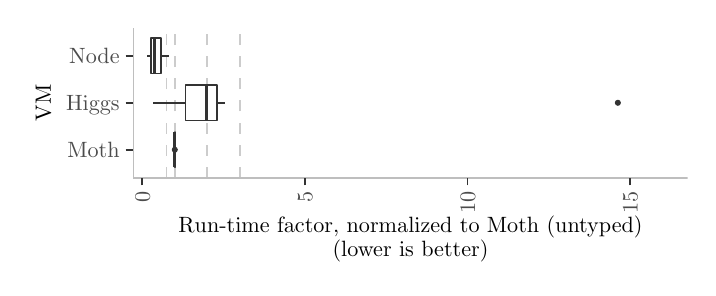
\begin{tikzpicture}[x=1pt,y=1pt]
\definecolor{fillColor}{RGB}{255,255,255}
\path[use as bounding box,fill=fillColor,fill opacity=0.00] (0,0) rectangle (238.49, 86.72);
\begin{scope}
\path[clip] ( 38.18, 32.44) rectangle (238.49, 86.72);
\definecolor{drawColor}{gray}{0.80}

\path[draw=drawColor,line width= 0.6pt,dash pattern=on 4pt off 4pt ,line join=round] ( 50.22, 32.44) -- ( 50.22, 86.72);

\path[draw=drawColor,line width= 0.6pt,dash pattern=on 4pt off 4pt ,line join=round] ( 53.16, 32.44) -- ( 53.16, 86.72);

\path[draw=drawColor,line width= 0.6pt,dash pattern=on 4pt off 4pt ,line join=round] ( 64.91, 32.44) -- ( 64.91, 86.72);

\path[draw=drawColor,line width= 0.6pt,dash pattern=on 4pt off 4pt ,line join=round] ( 76.65, 32.44) -- ( 76.65, 86.72);
\definecolor{drawColor}{gray}{0.20}
\definecolor{fillColor}{gray}{0.20}

\path[draw=drawColor,line width= 0.4pt,line join=round,line cap=round,fill=fillColor] ( 53.16, 42.62) circle (  0.89);

\path[draw=drawColor,line width= 0.6pt,line join=round] ( 53.16, 42.62) -- ( 53.16, 42.62);

\path[draw=drawColor,line width= 0.6pt,line join=round] ( 53.16, 42.62) -- ( 53.16, 42.62);
\definecolor{fillColor}{RGB}{255,255,255}

\path[draw=drawColor,line width= 0.6pt,line join=round,line cap=round,fill=fillColor] ( 53.16, 36.26) --
	( 53.16, 36.26) --
	( 53.16, 48.98) --
	( 53.16, 48.98) --
	( 53.16, 36.26) --
	cycle;

\path[draw=drawColor,line width= 1.1pt,line join=round] ( 53.16, 36.26) -- ( 53.16, 48.98);
\definecolor{fillColor}{gray}{0.20}

\path[draw=drawColor,line width= 0.4pt,line join=round,line cap=round,fill=fillColor] (213.26, 59.58) circle (  0.89);

\path[draw=drawColor,line width= 0.6pt,line join=round] ( 68.35, 59.58) -- ( 71.27, 59.58);

\path[draw=drawColor,line width= 0.6pt,line join=round] ( 57.06, 59.58) -- ( 45.44, 59.58);
\definecolor{fillColor}{RGB}{255,255,255}

\path[draw=drawColor,line width= 0.6pt,line join=round,line cap=round,fill=fillColor] ( 68.35, 53.22) --
	( 57.06, 53.22) --
	( 57.06, 65.94) --
	( 68.35, 65.94) --
	( 68.35, 53.22) --
	cycle;

\path[draw=drawColor,line width= 1.1pt,line join=round] ( 64.45, 53.22) -- ( 64.45, 65.94);

\path[draw=drawColor,line width= 0.6pt,line join=round] ( 48.26, 76.55) -- ( 51.20, 76.55);

\path[draw=drawColor,line width= 0.6pt,line join=round] ( 44.66, 76.55) -- ( 43.27, 76.55);

\path[draw=drawColor,line width= 0.6pt,line join=round,line cap=round,fill=fillColor] ( 48.26, 70.19) --
	( 44.66, 70.19) --
	( 44.66, 82.91) --
	( 48.26, 82.91) --
	( 48.26, 70.19) --
	cycle;

\path[draw=drawColor,line width= 1.1pt,line join=round] ( 45.99, 70.19) -- ( 45.99, 82.91);
\end{scope}
\begin{scope}
\path[clip] (  0.00,  0.00) rectangle (238.49, 86.72);
\definecolor{drawColor}{RGB}{190,190,190}

\path[draw=drawColor,line width= 0.6pt,line join=round] ( 38.18, 32.44) --
	( 38.18, 86.72);
\end{scope}
\begin{scope}
\path[clip] (  0.00,  0.00) rectangle (238.49, 86.72);
\definecolor{drawColor}{gray}{0.30}

\node[text=drawColor,anchor=base east,inner sep=0pt, outer sep=0pt, scale=  0.80] at ( 33.23, 39.87) {Moth};

\node[text=drawColor,anchor=base east,inner sep=0pt, outer sep=0pt, scale=  0.80] at ( 33.23, 56.83) {Higgs};

\node[text=drawColor,anchor=base east,inner sep=0pt, outer sep=0pt, scale=  0.80] at ( 33.23, 73.79) {Node};
\end{scope}
\begin{scope}
\path[clip] (  0.00,  0.00) rectangle (238.49, 86.72);
\definecolor{drawColor}{gray}{0.20}

\path[draw=drawColor,line width= 0.6pt,line join=round] ( 35.43, 42.62) --
	( 38.18, 42.62);

\path[draw=drawColor,line width= 0.6pt,line join=round] ( 35.43, 59.58) --
	( 38.18, 59.58);

\path[draw=drawColor,line width= 0.6pt,line join=round] ( 35.43, 76.55) --
	( 38.18, 76.55);
\end{scope}
\begin{scope}
\path[clip] (  0.00,  0.00) rectangle (238.49, 86.72);
\definecolor{drawColor}{RGB}{190,190,190}

\path[draw=drawColor,line width= 0.6pt,line join=round] ( 38.18, 32.44) --
	(238.49, 32.44);
\end{scope}
\begin{scope}
\path[clip] (  0.00,  0.00) rectangle (238.49, 86.72);
\definecolor{drawColor}{gray}{0.20}

\path[draw=drawColor,line width= 0.6pt,line join=round] ( 41.41, 29.69) --
	( 41.41, 32.44);

\path[draw=drawColor,line width= 0.6pt,line join=round] (100.15, 29.69) --
	(100.15, 32.44);

\path[draw=drawColor,line width= 0.6pt,line join=round] (158.89, 29.69) --
	(158.89, 32.44);

\path[draw=drawColor,line width= 0.6pt,line join=round] (217.64, 29.69) --
	(217.64, 32.44);
\end{scope}
\begin{scope}
\path[clip] (  0.00,  0.00) rectangle (238.49, 86.72);
\definecolor{drawColor}{gray}{0.30}

\node[text=drawColor,rotate= 90.00,anchor=base east,inner sep=0pt, outer sep=0pt, scale=  0.80] at ( 44.16, 27.49) {0};

\node[text=drawColor,rotate= 90.00,anchor=base east,inner sep=0pt, outer sep=0pt, scale=  0.80] at (102.91, 27.49) {5};

\node[text=drawColor,rotate= 90.00,anchor=base east,inner sep=0pt, outer sep=0pt, scale=  0.80] at (161.65, 27.49) {10};

\node[text=drawColor,rotate= 90.00,anchor=base east,inner sep=0pt, outer sep=0pt, scale=  0.80] at (220.39, 27.49) {15};
\end{scope}
\begin{scope}
\path[clip] (  0.00,  0.00) rectangle (238.49, 86.72);
\definecolor{drawColor}{RGB}{0,0,0}

\node[text=drawColor,anchor=base,inner sep=0pt, outer sep=0pt, scale=  0.80] at (138.33, 12.73) {Run-time factor, normalized to Moth (untyped)};

\node[text=drawColor,anchor=base,inner sep=0pt, outer sep=0pt, scale=  0.80] at (138.33,  4.09) {(lower is better)};
\end{scope}
\begin{scope}
\path[clip] (  0.00,  0.00) rectangle (238.49, 86.72);
\definecolor{drawColor}{RGB}{0,0,0}

\node[text=drawColor,rotate= 90.00,anchor=base,inner sep=0pt, outer sep=0pt, scale=  0.80] at (  8.36, 59.58) {VM};
\end{scope}
\end{tikzpicture}
